\section{Extraction des dates de semis par télédétection}
  
  \subsection{Considérations générales} \label{sec-general}
  
Les périodes ou dates les plus appropriés pour semer dépendent de nombreux facteurs.  Nous pouvons considérer les espèces et leurs variétés, les températures 
selon la zone de production, l'humidité du sol, les objectifs de la production (date de récolte souhaitée) ou encore les pratiques culturales (semi direct sans labour, semi en sec avant les premières pluies \ldots{}). Cependant, l'on peut
s'accorder sur le rôle prépondérant que joue le facteur climatique et plus précisement le début de la saison des pluies \citep{Ingram2002, Barbier2009}. En effet, au Sénégal comme dans d'autres pays d'Afrique où l'agriculture est pluviale, le comportement des agriculteurs est
généralement celui de semer après les premiers épisodes pluvieux importants \citep{Bacci1999}. Néanmoins, il existe un risque d'échec des premières semences en cas d'avènement d'une sécheresse \citep{Marteau2011} qui peut emmener les agriculteurs à semer de nouveau.\\ \'Etant donné l'étroite relation entre les rendements agricoles et la durée du cycle de développement des céréales comme le Mil, 
des semis tardifs sont susceptibles de 
conduire à des rendements faibles en fin de saison \citep{Sivakumar1990}. Le suivi du démarrage de la saison agricole permet donc de fournir aux décideurs, une évaluation précoce des menaces potentielles 
à la production agricole et à la sécurité alimentaire. L'une des méthodes les plus courantes pour l'estimation des dates de semis dans les pays d'Afrique de l'Ouest repose sur une approche agrométéorologique ou agroclimatiques
qui consiste à appliquer des seuils sur les quantités de précipitations survenues pendant une période définie \citep{Marinho2014}. Cependant, cette méthode est limitée par les inconvénients qu'elle présente : la résolution spatiale des données qui est souvent grossière (de l'ordre des kilomètres) et l'estimation en elle même des quantités de précipitations qui peut être imprécise. 
Compte tenu de notre échelle de travail qui est celle de la parcelle, cette méthode n'est pas adaptée à notre étude et ne peut être considérée. \\Une autre approche par télédection cette fois-ci
consiste à dériver les dates du début de croissance de la végétation ou en général les \emph{métriques phénologiques} à partir de séries temporelles d'indices de végétation comme le \acrshort{ndvi} ou le \acrshort{evi} 
et à en déduire les dates de semis. Ces indices de végétation rendent compte entre autres de l’activité photosynthétique de la
végétation, de l’intensité de son métabolisme ainsi que de sa verdure \citep{Duarte2018}. Cette approche par télédétection présente non seulement l'avantage d'avoir une résolution 
spatiale beaucoup plus élevée en fonction de l'image 
satellitaire utilisée mais d'intégrer également la réponse spectrale de la végétation aux divers facteurs externes comme les pratiques agricoles. Bien évidemment, les contraintes intrinsèques à
l'acquisition des images satellitaires ne sont pas en reste. C'est notamment le cas des bruits induits par la perturbations atmosphériques (nébulosité). Il faudra donc avant exploitation des images, considérer 
par exemple l'application d'une méthode de lissage. Une autre précaution est à prendre vis-à-vis de l'influence des sols nus dans la réponse spectrale du couvert végétal 
notamment quand celui ci est clairsemé tel pour des cultures peu couvrantes comme le Mil. Il faudra considérer par exemple l'utilisation d'un indice de végétation tenant compte de l'effet des sols comme le \acrshort{savi} ou le 
\acrshort{msavi}. Il existe une foultitude de méthodes dans la littérature pour estimer le démarrage de la végétation en étudiant sa phénologie par observation satellitaire. 
  
  \subsection{Phénologie de la végétation}
  
La \emph{phénologie} 
est l’étude de l’apparition d’événements périodiques (annuels le plus souvent) dans le monde vivant, déterminée par les variations saisonnières du climat. Elle se traduit au niveau de 
la végétation, par l’ensemble des stades de développement intervenant dans le cycle de vie des plantes en l’occurrence le bourgeonnement, la croissance, la floraison et la 
sénescence \citep{Kimball2014}. La phénologie du Mil peut être par exemple décomposée en une phase \emph{végétative}, une phase \emph{reproductrice} et une phase de 
\emph{maturation}. Selon les variétés de Mil cultivées, la longueur du cycle de développement peut être de 90 à 100 jours pour les \emph{Souna} (variétés à cycle court --- 
petits grains, épis non aristés et peu photosensibles) ou de 130 à 150 jours pour les \emph{Sanio} (variétés à cycle long --- grains plus gros, épis aristés et variété photopériodique) \citep{Diouf2001}.
\\L'\'etude de la phénologie des plantes sur une échelle régionale à globale à partir d’observations satellitaires est désignée par \acrfull{lsp} \citep{Helman2018}. Le terme LSP 
tient compte du fait que le signal intercepté par les satellites provient d’une surface hétérogène et n’est pas représentatif de la réponse spectrale d’une seule espèce 
\citep{Kimball2014}. L'analyse de la LSP contribue entre autres à diverses applications comme l’étude des changements climatiques \citep{Begue2014} ou encore au suivi des
cultures. Les séries temporelles d’indices de végétation provenant de capteurs à basse résolution comme AVHRR, MODIS, SPOT Vegetation ou encore PROBA-V permettent d’évaluer 
la phénologie de la végétation sur une échelle régionale à globale. Plus récemment, quelques auteurs ont étudié la phénologie de la végétation à une échelle beaucoup plus fine en utilisant des données
à haute et très haute résolution comme ceux du satellite chinois HJ-1 A/B \citep{Pan2015} ou du satellite RapidEye \citep{Vrieling2017}.

  \subsection{Métriques phénologiques}

Le démarrage de la croissance de la végétation et plus généralement les métriques phénologiques peuvent être utilisés comme proxy à l'évaluation des dates de semis. Les métriques phénologiques
ou variables phénologiques désignent l'ensemble des stades phénologiques du cycle saisonnier de la végétation dérivés par observation satellitaire \citep{Helman2018}. Elles fournissent 
donc des indications sur la dynamique des écosystèmes.
Il s'agit usuellement (\Cref{metrics}) : 
\begin{itemize}
 \item du démarrage de croissance de la végétation ou \acrshort{sos},
 \item du pic ou du maximum de croissance de la végétation \acrshort{pos},
 \item de la fin de croissance de la végétation \acrshort{eos},
 \item et de la durée de croissance de la végétation \acrshort{gsl} : différence de temps entre le SOS et le EOS.
\end{itemize}
Pour ces premières métriques citées, il importe de noter que l'on considère à la fois la date (jour exact dans l'année ou nombre de jours dans le cas du GSL) et la valeur de l'indice de 
végétation utilisé par exemple le NDVI. D'autres métriques en plus peuvent être également dérivées : 
\begin{itemize}
 \item le niveau de base (le plus bas) au cours du cycle de développement de la végétation
 \item le milieu de croissance de la végétation
 \item le taux de croissance de la végétation au début du cycle
 \item le taux de décroissance de la végétation à la fin du cycle
 \item la petite intégrale saisonnière (cumul du SOS au EOS pour les valeurs au dessus de la base)
 \item la grande intégrale saisonnière (cumul du SOS au EOS en totalité).
\end{itemize}

\begin{figure}[htbp]
 \begin{center}
  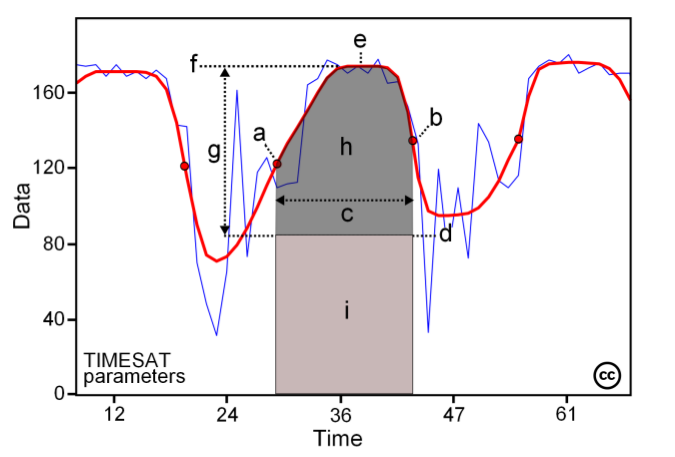
\includegraphics[scale=0.45]{synthese_biblio/metrics.png} 
 \end{center}
 \caption[Illustration de quelques métriques phénologiques]{Illustration de quelques métriques phénologiques : \emph{a- SOS b- EOS c- Durée de la saison d- Valeur de Base (en unité d'indice de végétation) e- Milieu de la saison f- Maximum de l'indice de végétation et g- Amplitude de l'indice de végétation}, Source : \citet{Eklundh2017}}
 \label{metrics}
\end{figure}
%\clearpage

Outre leur utilisation comme proxy à l'évaluation des dates de semis, les métriques phénologiques peuvent être employées à d'autres fins comme l'estimation de rendements, exploitant 
la forte corrélation avec la biomasse en fin de saison ou encore la détection d'anomalies dans le cycle de la végétation, en considérant une référence ou une normale parmi un 
historique de saisons culturales.

\vspace{5mm}

Comme évoqué dans la \cref{sec-general}, plusieurs méthodes ont été mises au point pour dériver les métriques phénologiques à partir de séries temporelles d'indices de végétation.
\citet{Beck2006} et \citet{Atzberger2013} les ont classé en 2 catégories : 
\begin{itemize}
 \item un premier groupe de méthodes qui estime le timing des transitions phénologiques de manière isolée et indépendante les unes des autres
 \item et un second groupe qui modélise la série temporelle entière par une fonction mathématique pour estimer les métriques phénologiques.
\end{itemize}
Dans le premier groupe, sont classées surtout les méthodes par seuillage sur les valeurs d'indices de végétation ou sur leurs amplitudes. Dans leur revue \citet{deBeurs2010} en ont décrit quelques unes comme la méthode par seuillage basée sur les ratios de NDVI \citep{White1997}. Les méthodes par seuillage sont les plus simples et les plus communes \citep{Pan2015}. En effet, elles supposent qu’un stade phénologique a commencé quand 
la valeur de l'indice de végétation atteint un certain seuil fixé \citep{Jonsson2002}. Cependant, cette approche peut s'avérer inconsistante quand le couvert végétal n'est 
pas homogène ou quand il s'agit d'écosystèmes cultivés avec plusieurs cycles culturaux au cours de l'année. De plus, un seuil n'est pas toujours transposable du fait qu'il soit bien souvent lié à sa zone d'application. La seconde catégorie regroupe les fonctions gaussiennes, les modèles logistiques et quadratiques \citep{Zhang2003,Jonsson2004}, l'analyse en composantes principales, l'analyse harmonique ou encore la transformation en ondelettes. Ces dernières méthodes sont plus poussées et plus complexes à mettre en \oe uvre. Il existe également une autre catégorie de méthodes dite de dérivées de courbes qui définissent généralement le SOS et le EOS respectivement comme les moments où l'on observe la plus grande hausse et la plus grande chute dans les valeurs de l'indice de végétation \citep{Moulin1997,Tateishi2004}.

\vspace{5mm}

Bon nombre de logiciels et applications ont été développés pour traiter les séries temporelles d'indices de végétation et en extraire les métriques phénologiques souhaitées. 
Nous avons identifié les suivants :
\begin{itemize}
 \item TIMESAT \footnote{\url{http://web.nateko.lu.se/timesat/timesat.asp?cat=0}} \citep{Eklundh2017} 
 \item SPIRITS \footnote{\url{http://spirits.jrc.ec.europa.eu/}}
 \item PhenoSat \footnote{\url{http://www.fc.up.pt/PhenoSat/software.html}} \citep{Rodrigues2013}
 \item Plugin QGIS QPhenoMetrics \citep{Duarte2018}
 \item Plugin QGIS VERSAO VegaMonitor \footnote{\url{https://github.com/Xdarii/VERSAO_VegaMonitor/wiki}}.
\end{itemize}

\section{Estimation des rendements par télédétection}
